\documentclass[11pt,a4paper]{article}
% ukazi za delo s slovenscino -- izberi kodiranje, ki ti ustreza
\usepackage[slovene]{babel}
%\usepackage[cp1250]{inputenc}
\usepackage[T1]{fontenc}
\usepackage[utf8]{inputenc}
\usepackage{amsmath,amssymb,amsfonts,amsthm}
\usepackage{url}
%\usepackage[normalem]{ulem}
\usepackage[dvipsnames,usenames]{color}
\usepackage{graphicx}
\usepackage{enumitem}
\usepackage{tikz}
%\usetikzlibrary{arrows.meta}
%\usetikzlibrary{shapes.geometric}
\usetikzlibrary{positioning}
\usepackage[parfill]{parskip}

% ukazi za matematicna okolja
\theoremstyle{definition} % tekst napisan pokoncno
\newtheorem{definicija}{Definicija}[section]
\newtheorem{primer}[definicija]{Primer}
\newtheorem{opomba}[definicija]{Opomba}

\renewcommand\endprimer{\hfill$\diamondsuit$}

\theoremstyle{plain} % tekst napisan posevno
\newtheorem{lema}[definicija]{Lema}
\newtheorem{izrek}[definicija]{Izrek}
\newtheorem{trditev}[definicija]{Trditev}
\newtheorem{posledica}[definicija]{Posledica}


% za stevilske mnozice uporabi naslednje simbole
\newcommand{\R}{\mathbb R}
\newcommand{\N}{\mathbb N}
\newcommand{\Z}{\mathbb Z}
\newcommand{\C}{\mathbb C}
\newcommand{\Q}{\mathbb Q}

% ukaz za slovarsko geslo
\newlength{\odstavek}
\setlength{\odstavek}{\parindent}
\newcommand{\geslo}[2]{\noindent\textbf{#1}\hspace*{3mm}\hangindent=\parindent\hangafter=1 #2}

% naslednje ukaze ustrezno popravi
\newcommand{\program}{Matematika} % ime studijskega programa: Matematika/Finan"cna matematika
\newcommand{\imeavtorja}{Ines Meršak} % ime avtorja
\newcommand{\imementorja}{prof.~dr. Sandi Klavžar} % akademski naziv in ime mentorja
\newcommand{\naslovdela}{Problem londonskega stolpa}
\newcommand{\letnica}{2016} %letnica diplome


% commands
\newcommand{\graf}[1][G]{\ensuremath{#1 = (V(#1), E(#1))}}
\newcommand{\vozlisca}[1][G]{\ensuremath{V(#1)}}
\newcommand{\povezave}[1][G]{\ensuremath{E(#1)}}
\newcommand{\bd}{\ensuremath{|\,}}
\newcommand{\ed}{\ensuremath{\,|}}
% operatorji
\DeclareMathOperator {\stopnja} {deg}

\title{Problem londonskega stolpa}
\author{Ines Meršak}
\date{13.~05.~2016}


\begin{document}

\maketitle

 
% tu se zacne tekst seminarja
\section{Klasični problem Londonskega stolpa}

\begin{itemize}
    \item izumil Tim Shallice, profesor nevropsihologije, leta 1982
    \item tri enako velike krogle različnih barv
    \item tri palice različnih velikosti
    \item na prvo palico lahko postavimo samo eno kroglo, na drugo le dve krogli, na tretjo pa tri
    \item cilj igre je priti iz nekega danega stanja v neko drugo želeno stanje z minimalnim številom potez
\end{itemize}
    
Stanja (in prehode med njimi) lahko elegantno opišemo s pomočjo teorije grafov.

\subsection{Osnovne definicije teorije grafov}

\begin{itemize}
	\item \emph{graf} $G$ je urejen par $(\vozlisca, \povezave)$, kjer je $\vozlisca$ končna množica \emph{vozlišč}, $\povezave$ pa množica \emph{povezav} grafa (neurejeni pari vozlišč)
    \item $u$ in $v$ sta \emph{sosednji vozlišči}, če obstaja povezava med njima
	\item \emph{soseščina} vozlišča $u$ je množica vseh sosednjih vozlišč vozlišča $u$:
	\( N(u) = \{ x\colon ux \in \povezave \} .\)
	\item \emph{stopnja vozlišča} $u$ je število vseh vozlišč, ki so mu sosednji: $\stopnja u = |N(u)|$.
    \item \emph{sprehod} v grafu $G$ je zaporedje vozlišč $v_1, v_2, \ldots, v_k$, tako da velja $v_i v_{i+1} \in E(G),$ pri čemer je $1 \leq i \leq k-1$
    \item graf je \emph{povezan}, če za poljuben par vozlišč obstaja sprehod med njima
    \item \emph{razdalja} $d_G(u,v)$ med poljubnima vozliščema $u$ in $v$ v povezanem grafu $G$ je najmanjše možno število povezav na nekem sprehodu, ki se začne v $u$ in konča v $v$
    \item \emph{premer} grafa je največjo minimalna razdalja med pari vozlišč; če vzamemo poljubno vozlišče v grafu, potem lahko pridemo do drugega poljubnega vozlišča preko $d$ ali manj povezav, kjer je $d$ premer grafa
    \item graf je \emph{ravninski}, če ga lahko narišemo v ravnini tako, da se nobeni povezavi ne križata
    \item \emph{pot} na $n$ vozliščih je graf, ki ima dve vozlišči stopnje $1$, medtem ko so preostala vozlišča stopnje $2$
    \item \emph{cikel} na $n$ vozliščih je graf, ki ga dobimo iz poti na $n$ vozliščih tako, da dodamo povezavo med vozliščema stopnje $1$
    \item \emph{Hamiltonova pot} je pot v grafu, ki vsebuje vsa vozlišča
    \item \emph{Hamiltonov cikel} nekega grafa $G$ je cikel v $G$, ki poteka skozi vsa vozlišča tega grafa

\end{itemize}

\subsection{Graf klasičnega problema londonskega stolpa}
Označimo krogle s številkami 1, 2, 3, pri čemer je npr.\ krogla 1 modra, krogla 2 rdeča, krogla 3 pa rumena. Začetek naslednje palice bomo nakazali z |, krogle pa bomo naštevali od vrha proti dnu palice.
Na primer: stanja na prejšnji sliki so |3|12 in |21|3.
Vidimo, da je minimalno število potez pri tem primeru 4 in da obstaja samo eno najkrajše zaporedje potez.
S pomočjo teh oznak lahko opišemo vsako možno stanje in narišemo graf londonskega stolpa, pri čemer so vozlišča stanja, povezave pa so med tistimi stanji, med katerimi lahko prehajamo z eno potezo (enim veljavnim premikom krogle).

\begin{figure}[h]
    \centering
    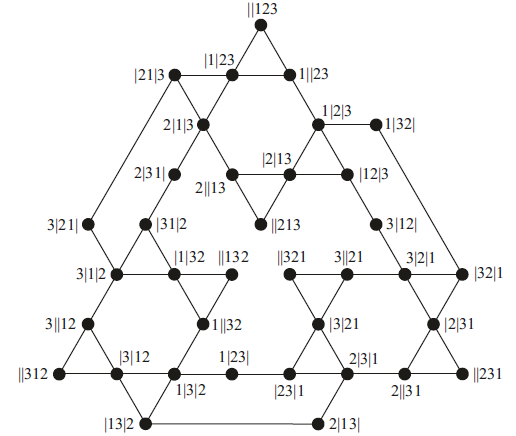
\includegraphics[height=200pt]{../img/tolgraph.png}
\end{figure}

%\begin{lema}
%    \label{lem:stanja-klas-lond}
%    Število vseh možnih stanj klasičnega londonskega stolpa je 36.
%\end{lema}

\begin{itemize}
    \item 36 vozlišč (sledi iz leme~\ref{lem:stanja-klas-lond})
    \item 12 vozlišč stopnje 2, 3, 4
    \item premer grafa je 8
    \item ravninski (narisan je v ravnini, povezave se nikjer ne križajo)
\end{itemize}

\begin{trditev}
    Graf $L$ vsebuje Hamiltonovo pot, ne pa tudi Hamiltonovega cikla.
\end{trditev}

\begin{proof}
    TODO
    
    Hitro lahko dokažemo, da $L$ vsebuje Hamiltonovo pot: poiščemo jo. Ena izmed Hamiltonovih poti v grafu $L$ je prikazana na sliki~\ref{}.
    
    Da bi dokazali, da graf ni Hamiltonov, moramo najprej opaziti nekaj lastnosti tega grafa. Soseščina vsakega vozlišča stopnje 2 je sestavljena iz enega vozlišča stopnje 3 in enega stopnje 4, prav tako je presek soseščin poljubnih dveh vozlišč stopnje 2 prazen -- vsako vozlišče stopnje 2 ima torej ``svoje'' vozlišče stopnje 3 in stopnje 4. Nadalje lahko iz grafa vidimo, da poljubni dve vozlišči stopnje 3 nista sosednji.
    
    Sledi, da na ciklu $C$ v grafu, ki bi vseboval vsa vozlišča, nobeni dve vozlišči stopnje 4 nista sosednji. Ker imamo po 12 vozlišč vsake stopnje, bi v nasprotnem primeru namreč prišli do zaključka, da morata biti sosednji dve vozlišči stopnje 3, kar pa je v protislovju z zgornjim opažanjem.
    
    Sedaj začnimo graditi cikel $C$, ki bo vseboval vsa vozlišča grafa natanko enkrat. Oglejmo si sliko~\ref{}.
    Cikel $C$ mora torej gotovo iti skozi vsa vozlišča stopnje 2, kar je možno le na en način: če imamo vozlišče stopnje 2 $v$ s sosedoma $u$ stopnje 3 in $z$ stopnje 4, mora $C$ vsebovati pot $u,v,z$.
    Če začnemo pri vozlišču stopnje 2 $||\,123$, mora graf torej vsebovati pot $1||23, ||123, |1|23$. Slednje je vozlišče stopnje 4, za nadaljevanje cikla pa imamo dve možnosti: vozlišče $2|1|3$ ali $|21|3$. Ker je prvo stopnje 4 in smo že prej opazili, da dve vozlišči iste stopnje ne bosta sosednji na ciklu $C$, cikel nadaljujemo z $|21|3$. Sosed tega vozlišča je vozlišče $3|21|$ stopnje 2, zato moramo cikel gotovo nadaljevati skozi njega. Pridemo do vozlišča $3|1|2$. Imamo dve možnosti: 
    \begin{itemize}[label={-}]
        \item Nadaljujemo z vozliščem $|31|2$, ki je stopnje 3 in je na notranjem ciklu. V tem primeru ne bomo notranjega cikla nikoli zapustili, saj je notranji cikel oblike: vozlišče stopnje 2, vozlišče stopnje 3 (povezano samo z vozlišči na notranjem ciklu), vozlišče stopnje 4, ki je nato povezano z vozliščem stopnje 2, skozi katerega moramo iti. Nato pa sledita vozlišče $a$ stopnje 3 (povezano z notranjim ciklom in vozliščem stopnje $w$ 4 na zunanjem ciklu) in vozlišče $b$ stopnje 4 (povezan z vozliščem $c$ stopnje 2 in še dvema drugima na notranjem ciklu ter vozliščem $w$). Ker moramo iti skozi vozlišče $c$, moramo tudi skozi $b$, od prej pa vemo, da moramo nujno tudi skozi $a$, saj je sosed vozlišča stopnje 2. Torej lahko pot speljemo le skozi $a,b,c$, saj je $w$ stopnje 4 in na ciklu zato ne sme biti soseden $b$, ki je prav tako stopnje 4.
        \item Pot torej nadaljujemo z vozliščem stopnje 3 na zunanjem ciklu $3||12$, in tudi v nadaljevanju ostanemo na zunanjem ciklu, saj vemo, da bomo v nasprotnem primeru ostali na notranjem ciklu.
    \end{itemize}
    Torej ne moremo konstruirati cikla, bi vseboval vsa vozlišča našega grafa $L$ natanko enkrat. $L$ torej ni Hamiltonov.
    \qedhere
\end{proof}


\section{Posplošeni londonski stolp}
Graf klasičnega problema je majhen, možnih stanj je malo, zato je za testiranje odraslih ljudi naloga včasih prelahka; Jenny R.\ Tunstall je prva predlagala razširitev na 4 krogle s podaljšanimi palicami (vsaka je podaljšana za eno enoto).

\subsection{Definicija}

Poglejmo si posplošitev tega problema na $p$ palic in $n$ krogel različne barve, pri čemer je $p \geq 3 \text{ in } n \geq 2$. Vsako palico označimo s številom $k \in [p]$, pri čemer je $h_k$ višina palice (ta predstavlja število krogel, ki jih drži palica). Krogle označimo z 1 do $n$ -- te lahko razporejamo na palice. Veljati mora $n \leq \sum_{k=1}^p h_k$. Poteza je veljavna, če vrhnjo kroglo neke palice prestavimo na vrh druge, pod pogojem, da je na tej palici manj kot $h_k$ krogel.

Vsako stanje krogel lahko enolično predstavimo s permutacijo $s \in S_{n+p}$, $S$ je simetrijska grupa. Pri tem je $s_i$ položaj krogle $i$, če $i \in [n] $, ali dna palice $i-n$, če je $i \in [n+p] \setminus [n] $. Položaje oštevilčimo od leve palice proti desni, z vrha palice proti dnu (kot pri klasičnem problemu). Tako bo s številko 1 oštevilčen položaj krogle, ki je postavljena najvišje na prvi palici; če na prvi palici ni nobene krogle, bo imelo položaj 1 dno te palice.

Naš primer: $s = 452136$.
{\small $s$ bomo zapisali v obliki $ \sum_1 | \ldots | \sum_p $, kjer je $\sum_k$ niz oznak krogel v položajih od $s_{n+k-1} + 1$ do $s_{n+k}-1$ od vrha palice navzdol. $s_{n+0} = 0$ in ne $s_n$. Vertikalne pipe spet označujejo začetek dna palice.}

\begin{definicija}
    \emph{Londonski graf} $L_h^n$, kjer je $p \geq 3,\ n \geq 2,\ h \in [n]^p,\  \sum_{k=1}^p h_k \geq n$:
    \begin{itemize}
        \item vozlišča: vse permutacije $s \in S_{n+p}$, za katere velja:
        \[\forall k \in [p]:\ 1 \leq s_{n+k} - s_{n+k-1} \leq h_k + 1,\ s_{n+p} = n + p ,\]
        \item povezave: vsaki dve stanji (oz.\ pripadajoči permutaciji), med katerima lahko prehajamo z veljavno potezo, sta povezani
    \end{itemize}
\end{definicija}

Hitro vidimo, da mora veljati 
\[\forall k \in [p]\colon s_{n+k} - s_{n+k-1} \geq 1 \]
saj je $s_{n+k}$ položaj dna palice $k$, $s_{n+k-1}$ pa položaj dna palice $k-1$, torej se mora njun položaj razlikovati najmanj za 1 -- to se zgodi, če na palici $k$ ni nobene krogle.

Prav tako pa mora veljati tudi 
\[\forall k \in [p]\colon s_{n+k} - s_{n+k-1} \leq h_k + 1,\]
kar se zgodi v primeru, če je na $k$-ti palici $h_k$ krogel.

S pogojem, da so vse palice visoke največ $n$, ne izgubimo splošnosti, saj razporejamo le $n$ krogel.

Če smo v primeru klasičnega londonskega stolpa lahko izračunali število vozlišč, pa je v splošnem za londonske stolpe to precej težko. Kasneje bom obravnavala poseben primer londonskih grafov, za katerega je znana formula za število vozlišč. 

\subsection{Povezanost}
Zaželjeno je, da lahko pri londonskem stolpu prehajamo med poljubnima dvema stanjema, saj se problem uporablja za psihološka testiranja. To velja, če je pripadajoči londonski graf povezan, kar je zato ena pomembnejših lastnosti tega grafa.

V nadaljevanju bomo privzeli, da so palice urejene po velikosti naraščajoče, velja torej $h_1 \leq h_2 \leq \cdots \leq h_p$.
Potreben pogoj za povezanost londonskega grafa je očitno 
\[ n \leq \sum_{k=1}^{p-1} h_k, \]
oziroma z besedami, da lahko krogle razporedimo tako, da najvišja palica ostane prazna. V nasprotnem primeru bi, po tem ko bi razporedili maksimalno možno število krogel na vse preostale (manjše) palice, na največji ostalo še nekaj krogel, ki jih nikoli ne bi mogli premakniti na kakšno drugo palico.
Izkaže se, da je ta pogoj tudi zadosten za povezanost londonskega grafa.

\begin{izrek}
    Londonski graf $L_h^n$ je povezan natanko tedaj, ko velja pogoj
    \begin{equation}
        n \leq \sum_{k=1}^{p-1} h_k.
        \label{eq:pogoj-povezanosti}
    \end{equation}
\end{izrek}

\begin{proof}
    Želimo dokazati, da iz pogoja \eqref{eq:pogoj-povezanosti} sledi, da lahko najdemo pot med poljubnima dvema vozliščema v londonskem grafu, kar je ravno definicija povezanosti. Dokaza se lotimo tako, da poskušamo splošen problem čim bolj zreducirati.
    
    Predpostavili bomo, da je število vseh krogel enako kar vsoti višin vseh palic brez največje, saj lahko v nasprotnem primeru vpeljemo navidezne krogle, katerih premike kasneje zanemarimo. Velja naj torej $n = \sum_{k=1}^{p-1}h_k$.
    
    Spomnimo se, da vsako vozlišče grafa predstavlja neko stanje krogel -- če torej iščemo pot v grafu med dvema vozliščema, pravzaprav rešujemo problem, kako iz začetnega stanja krogel priti v končno. Predpostavimo lahko, da je tako pri začetnem kot tudi pri končnem stanju krogel največja palica prazna. V nasprotnem primeru jih lahko na začetku razporedimo na preostale palice, na koncu pa preprosto prestavimo na največjo palico.
    
    Sedaj postopamo tako, da izberemo kroglo, ki še ni na svojem (končnem) položaju, in jo zamenjamo s kroglo, ki se trenutno nahaja na tem položaju; ta postopek ponavljamo. Če lahko zamenjavo naredimo tako, da se pri tem ne spremeni položaj nobene druge krogle, je po koncu zamenjave še ena krogla več na pravem mestu.
    Ker je največja palica prazna, vse druge pa zapolnjene, se po koncu ponavljanja tega postopka ne more zgoditi, da je le ena krogla na napačnem mestu. (TODO zakaj?)
    
    Predpostavimo lahko še, da je ena izmed krogel, ki ju bomo zamenjali, na vrhu prve, najmanjše, palice. Namreč, s tremi zamenjavami, pri katerih je ena izmed krogel vedno na vrhu prve palice, lahko nadomestimo splošno zamenjavo dveh poljubnih krogel.
    
    Sedaj si izberimo kroglo, ki ni na pravem položaju, in s tem tudi kroglo, ki je trenutno na njenem položaju. Predpostavili smo, da je ena izmed teh krogel na prvi palici -- to kroglo označimo z $a$, drugo pa z $b$. Ločimo dva primera:
    
    \begin{enumerate}
        \item \textbf{Krogla $b$ je na prvi palici.}
        Vrhnjo kroglo druge palice, označimo jo s $c$, premaknemo na največjo ($p$-to) palico. Nato kroglo $a$ premaknemo na vrh druge palice, preostale krogle na prvi palici z do vključno kroglo $b$ pa premaknemo (seveda eno naenkrat) na največjo palico. Krogla $a$ lahko sedaj zasede svoj pravi položaj na prvi palici, $b$ pa premaknemo iz vrha največje palice na vrh druge. Sedaj lahko vrnemo vse preostale krogle (razen $c$) na prejšnje mesto na prvi palici, nato lahko na vrh prve palice postavimo $b$, ki tako zavzame prejšnji položaj krogle $a$. Za konec premaknemo še kroglo $c$ z največje palice na vrh druge palice.
        \item \textbf{Krogla $b$ ni na prvi palici.}
        V tem primeru je postopek še nekoliko lažji: najprej vse krogle nad $b$ premaknemo na največjo palico, nato na vrh največje palice premaknemo tudi $b$. Sedaj lahko kroglo $a$ prestavimo na njeno pravo mesto (kjer je bil prej $b$), $b$ na vrh prve palice, vse preostale krogle na največji palici pa postavimo nazaj na prejšnja mesta, nad kroglo $a$.
    \end{enumerate}
    S tem je dokaz končan, saj smo našli način, kako prehajati med dvema poljubnima stanjema krogel, in smo s tem našli tudi pot v grafu med poljubnima vozliščema.
\end{proof}

\subsection{Ravninskost}
\begin{itemize}
    \item operacija \emph{subdivizije} ohranja ravninskost: vzamemo neko povezavo $e$ grafa $G$ in na sredino te povezave dodamo še eno vozlišče 
    \item graf $H$ je \emph{subdivizija} grafa $G$, če ga lahko dobimo iz $G$ z zaporednim \emph{subdiviziranjem} povezav grafa $G$; očitno je tak $H$ ravninski natanko tedaj, ko je $G$ ravninski
    \item hitro lahko vidimo, da grafa $K_5$ in $K_{3,3}$ nista ravninska (poskusimo ju narisati v ravnini, a kmalu ugotovimo, da to ne bo mogoče)
    \item graf torej zagotovo ni ravninski, če vsebuje subdivizijo $K_5$ ali $K_{3,3}$; zanimivo pa je, da velja tudi obratno; dokaz tega dejstva je netrivialen in ga bom preskočila
\end{itemize}

\begin{izrek}[Kuratowski]
    Graf G je ravninski natanko tedaj, ko ne vsebuje subdivizije $K_5$ niti subdivizije $K_{3,3}$.
\end{izrek}

\begin{trditev}
    Naj bo $p=3$. Tedaj so londonski grafi $L_h^2, L_{122}^3,L_{123}^3$ in $ L_{133}^3$ ravninski.
\end{trditev}


\section{Oxfordski graf}

\emph{Oxfordski graf} je poseben primer londonskega grafa, za katerega velja, da so vse palice velikosti $n$, pri čemer je $n$ število krogel. Oxfordski graf označimo z $O^n_p$, zanj torej velja $O^n_p := L^n_{n^p}$.

Medtem ko je v splošnem težko določiti število vozlišč londonskega grafa, pa je to precej bolj preprosto za oxfordski graf. Še več, določimo lahko tudi število povezav.

\begin{trditev}
	Število vozlišč oxfordskega grafa $O^n_p$ je enako \[\frac{(n+p-1)!}{(p-1)!}.\]
\end{trditev}

\begin{proof}
	Iščemo število vseh možnih stanj pri oxfordskemu stolpu, saj je to enako številu vozlišč oxfordskega grafa.
	Podobno kot pri dokazu števila stanj klasičnega londonskega stolpa najprej pozabimo na različne barve krogel (delamo se, da so krogle enake) in se osredotočimo samo na njihovo postavitev. 
	
	Na koliko načinov lahko $n$ enakih krogel razvrstimo na $p$ palic višine $n$? Pri tem nimamo nobenih omejitev, saj so palice dovolj visoke, da lahko vse krogle postavimo tudi na eno samo palico. Lahko si predstavljamo, da imamo vse krogle zložene v vrsto, označene naj bodo z 0, nato pa na poljubna mesta (s ponavljanjem) vrivamo 1, ki naj pomeni konec neke palice in začetek neke druge. Ko vrinemo $p-1$ enic, smo določili $p$ palic in s tem razporeditev krogel. 
	
	Sedaj lahko na problem pogledamo malo drugače: na $n+p-1$ mest razporejamo $n$ ničel, ki predstavljajo krogle, in $p-1$ enic, ki predstavljajo začetek nove palice. Če razporedimo vse enice, bodo na vsa preostala mesta prišle ničle, razporeditev bo s tem določena. $p-1$ mest izmed $n+p-1$ položajev lahko izberemo na ${n+p-1 \choose p-1}$ načinov. S tem je položaj krogel na palicah točno določen, torej imamo ${n+p-1 \choose p-1}$ vseh možnih razporeditev, če privzamemo, da so krogle enake. 
	
	Ker je vsaka krogla drugačne barve, imamo za vsako razporeditev še $n!$ možnih permutacij barv. Število vseh stanj, in zato tudi število vozlišč, je tako enako
	
	\[ n! \cdot {n+p-1 \choose p-1} = n! \cdot \frac{(n+p-1)!}{n!(p-1)!} = \frac{(n+p-1)!}{(p-1)!}. \] \qedhere
\end{proof}

Pred dokazom formule za število povezav bomo potrebovali osnovno lemo teorije grafov, s pomočjo katere lahko na enostaven način izračunamo število povezav tega grafa, če imamo podano stopnjo vseh vozlišč grafa.

\begin{lema}[Lema o rokovanju]
    \label{lema:rokovanje}
    Za vsak graf \graf velja formula
    \begin{equation}
    \sum_{u \in V(G)}\! \stopnja u = 2 \cdot |E(G)|.
    \label{eq:lema-o-rokovanju}
    \end{equation}
\end{lema}

\begin{proof}
    Naredimo si tabelo vozlišč in povezav:
    
    \begin{table}[h]
        \centering
        \begin{tabular}{c|ccc}
            & \ldots & $e_j$ & \ldots \\ \hline
            \vdots & & \vdots & \\
            $v_i$ & \ldots & 1 / 0 & \\
            \vdots & & &
        \end{tabular}
    \end{table}
    
    V prvem stolpcu so našteta vozlišča grafa, v prvi vrstici pa povezave. Na mestu $i,j$ v tabeli zapišemo enico, če je vozlišče $v_i$ eno izmed krajišče povezave $e_j$, in ničlo v nasprotnem primeru. 
    
    Vemo, da ima vsaka povezava dve krajišči, torej sta v vsakem stolpcu natanko dve enici. Če po drugi strani pogledamo število enic v neki vrstici $i$, nam to pove ravno stopnjo vozlišča $v_i$. Ker mora biti rezultat enak, če seštejemo ničle in enice po stolpcih oziroma po vrsticah, sledi formula \eqref{eq:lema-o-rokovanju}.
\end{proof}

Pred dokazom formule za število povezav Oxfordskega grafa si na hitro oglejmo še dve lastnosti binomskih simbolov, ki ju bomo potrebovali v dokazu:

\begin{equation}
    \label{eq:binom}
    {b+w \choose l} = \sum_{k=0}^{l}{b \choose k}{w \choose l-k}
\end{equation}

\begin{trditev}
	Število povezav oxfordskega grafa $O^n_p$ je enako
	\[ \frac{np}{2} \frac{(p-2+n)!}{(p-2)!} .\]
\end{trditev}

\begin{proof}
    Vzemimo stanje (vozlišče), pri katerem je $q$ palic nepraznih, $1 \leq q \leq p$ in $n \geq q$. Vsako vrhnjo kroglo ene izmed $q$ palic lahko premaknemo na katerokoli palico, razen trenutne; izberemo torej eno izmed $q$ palic, s katere premaknemo kroglo, in eno izmed preostalih $p-1$ palic, kamor kroglo premaknemo. Tako vozlišče je torej stopnje $q(p-1)$. (Pri tem upoštevamo, da je povezava med dvema vozliščema grafa pravzaprav veljavna poteza med dvema stanjema.)
    
    Vseh stanj, ki imajo točno $q$ nepraznih palic, je enako
    \[{p \choose q} \frac{n!}{(n-q)!} \cdot |V(O^{n-q}_q)|.\]
    Najprej izberemo $q$ izmed $p$ palic, ki bodo neprazne, kar lahko storimo na ${p \choose q}$ načinov. Na vsako izmed teh $q$ palic moramo nujno postaviti vsaj eno kroglo, kar lahko naredimo na $n \cdot (n-1) \cdot \ldots \cdot (n-q+1) = \frac{n!}{(n-q)!}$ (za prvo izmed $q$ palic imamo na voljo $n$ krogel, za drugo $n-1$ krogel,\ldots). Preostalih $n-q$ krogel pa lahko razporedimo poljubno na $q$ palic, kar je brez škode za splošnost enako številu razporeditev $n-q$ krogel na $q$ palic velikosti $n-q$, torej $|V(O^{n-q}_q)|$.
    Če uporabimo formulo za število vozlišč oxfordskega grafa~\eqref{eq:oxford-vozl} in poračunamo, dobimo, da je število takih stanj enako
    \begin{align*}
    {p \choose q} \frac{n!}{(n-q)!} \cdot |V(O^{n-q}_q)| &=
    {p \choose q} \frac{n!}{(n-q)!} \frac{(n-q+q-1)!}{(q-1)!} \\ &= n! {p \choose q} \frac{(n-1)!}{(q-1)!\,(n-q)!} \\ &=
    n! {p \choose q} {n-1 \choose q-1}
    \end{align*}
    
    Sedaj po $q$ seštejemo stopnje vseh vozlišč (upoštevamo, da imajo vsa vozlišča, kjer je nepraznih točno $q$ palic, enako stopnjo) in uporabimo formulo~\eqref{eq:lema-o-rokovanju} iz leme o rokovanju:
    \begin{align*}
    |E(O^n_p)|
    &= \frac{1}{2} \sum_{q=1}^{p} \overbrace{q(p-1)}^{\text{stopnja vozlišča}} 
    \overbrace{n! {p \choose q} {n-1 \choose q-1} }^{\text{št.~vozlišč s to stopnjo}} \\
    &= \frac{1}{2} (p-1) n! \sum_{q=1}^{p} q {p \choose q} {n-1 \choose q-1} \\
    &= \frac{1}{2} (p-1) n! \sum_{q=1}^{p} q \frac{p!}{q! \, (p-q)!} {n-1 \choose q-1} \\
    &= \frac{1}{2} (p-1) n! \sum_{q=1}^{p} p \frac{(p-1)!}{(q-1)! \, (p-q)!} {n-1 \choose q-1} \\
    &= \frac{1}{2} p (p-1) n! \sum_{q=1}^{p} {p-1 \choose q-1} {n-1 \choose q-1}
    \end{align*}
    Sedaj uvedemo nov indeks $k = q-1$, upoštevamo lastnosti binomskih simbolov in uporabimo formulo~\eqref{eq:binom}:
    \begin{align*}
    |E(O^n_p)|
    &= \frac{1}{2} p (p-1) n! \sum_{k=0}^{p-1} {p-1 \choose k} {n-1 \choose k} \\
    &= \frac{1}{2} p (p-1) n! \sum_{k=0}^{p-1} {p-1 \choose p-1-k} {n-1 \choose k} \\
    &= \frac{1}{2} p (p-1) n! {p-1 + n-1 \choose p-1} \\
    &= \frac{1}{2} p (p-1) n! {n + p - 2 \choose p-1} \\
    &= \frac{1}{2} p (p-1) n! \frac{(n+p-2)!}{(p-1)!\,(n-1)!} \\
    &= \frac{1}{2} p n \frac{(n+p-2)!}{(p-2)!} \\
    &= \frac{np}{2} \frac{(p-2+n)!}{(p-2)!} \qedhere
    \end{align*}
\end{proof}

% seznam uporabljene literature
\begin{thebibliography}{99}

\bibitem{bib:tohmyths} A. M. Hinz, S. Klavžar, U. Milutinović in C. Petr, \emph{The Tower of Hanoi – Myths and Maths}, Birkhäuser, Basel, 2013.

\bibitem{bib:potocnik} P. Potočnik, \emph{Zapiski predavanj iz Diskretne Matematike I}, 1.~izdaja, [ogled 29.~12.~15], dostopno na \url{http://www.fmf.uni-lj.si/~potocnik/Ucbeniki/DM-Zapiski2010.pdf}

\bibitem{bib:wikishal} \emph{Tim Shallice}, v: Wikipedia: The Free Encyclopedia, [ogled 8.~10.~2015], dostopno na\\ \url{https://en.wikipedia.org/wiki/Tim_Shallice}.

\bibitem{bib:wikihamilpath} \emph{Hamiltonian path}, v: Wikipedia: The Free Encyclopedia, [ogled 28.~12.~2015], dostopno na \url{https://en.wikipedia.org/wiki/Hamiltonian_path}.
\end{thebibliography}

\end{document}

